\section{All about Computer}
\label{sec:computer}
\begin{frame}<beamer>
    \frametitle{Outline}
    \tableofcontents[currentsection]
\end{frame}

\begin{frame}
\frametitle{About Computer (1)}
\begin{itemize}
	\item {What is computer?}
	\begin{itemize}
		\item {Machine for computation}
		\item {Essentially, no big difference from abacus}
		\item {In our history, we have several kinds of machines used for computing}
		\begin{itemize}
			\item {Abacus}
			\item {Difference engine}
			\item {Tide-predicting machine}
		\end{itemize}
	\end{itemize}
\end{itemize}
\begin{figure}
	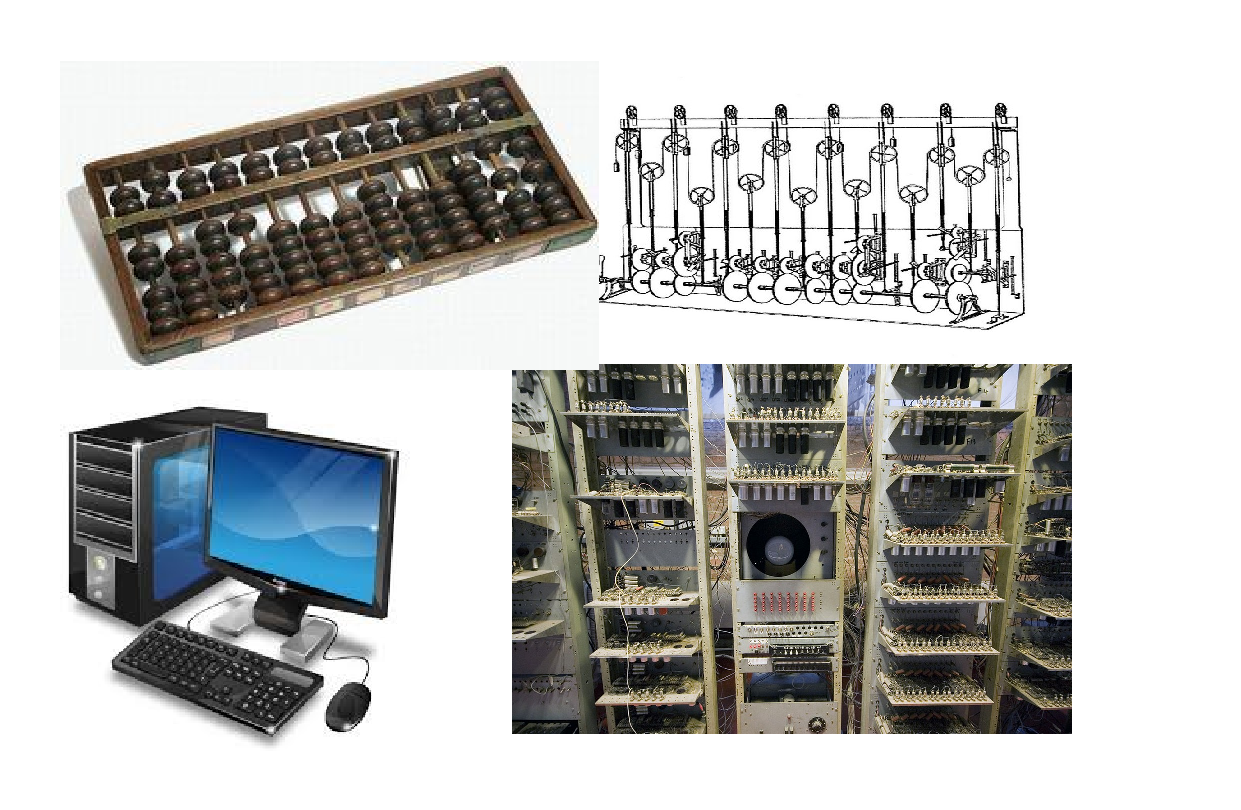
\includegraphics[width=0.5\linewidth]{figs/history_pcs.pdf}
\end{figure}
\end{frame}

\begin{frame}
\frametitle{About Computer (2): the model}
\begin{itemize}
	\item {What is computing}
	\begin{itemize}
		\item {Input data and needed operations}
		\item {Output the answer}
	\end{itemize}
	\begin{itemize}
		\item {This is actually the model proposed by \textbf{Alan Turing}}
	\end{itemize}
\end{itemize}
\begin{figure}
	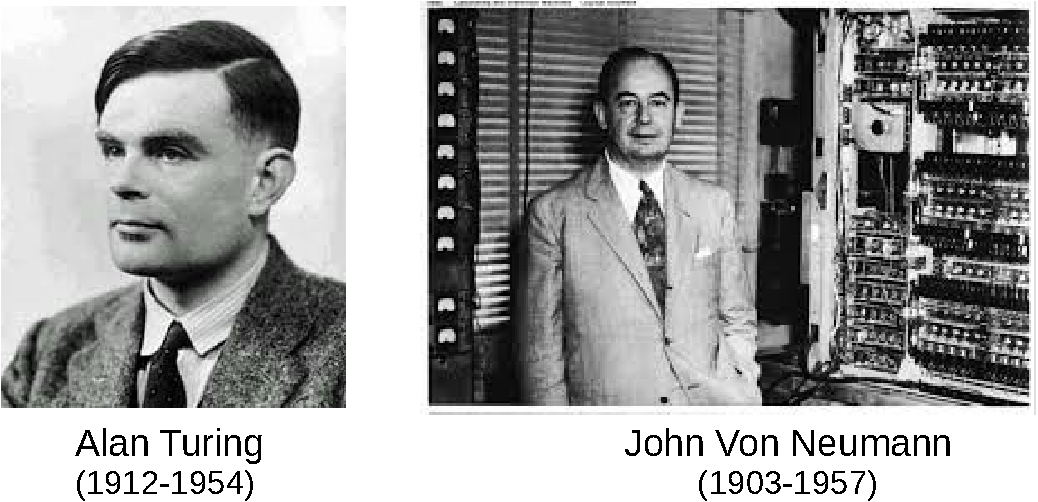
\includegraphics[width=0.8\linewidth]{figs/turing.pdf}
\end{figure}
\end{frame}

\begin{frame}
\frametitle{About Computer (3): the framework}
\begin{itemize}
	\item {Think aloud about the major components of a computer}
	\begin{itemize}
		\item {CPU: central processing unit}
		\item {Memory}
		\item {Hard disc}
		\item {Keyboard}
		\item {graphics card+Monitor/screen}
		\item {Music card+microphone+speaker}
		\item {Mouse}
	\end{itemize}
\end{itemize}
\begin{figure}
	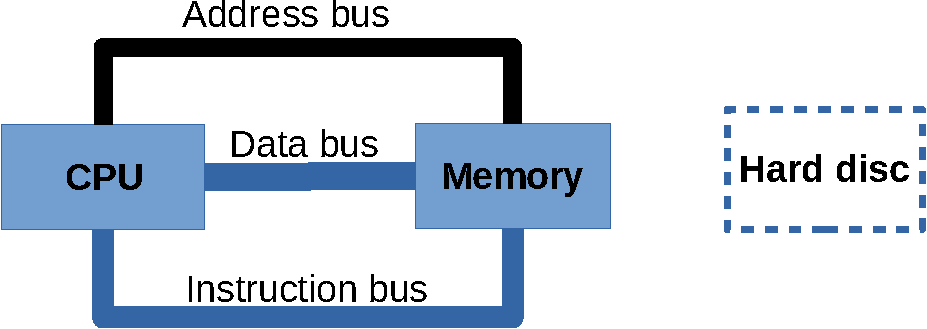
\includegraphics[width=0.7\linewidth]{figs/framework.pdf}
\end{figure}
\end{frame}

\begin{frame}
\frametitle{About Computer (4): the framework}
\begin{itemize}
	\item {Think aloud about the major components of a computer}
	\begin{itemize}
		\item {\textbf{CPU: central processing unit}}
		\item {\textbf{Memory}}
		\item {Hard disc}
		\item {Keyboard}
		\item {graphics card+Monitor/screen}
		\item {Music card+microphone+speaker}
		\item {Mouse}
	\end{itemize}
\end{itemize}
\begin{figure}
	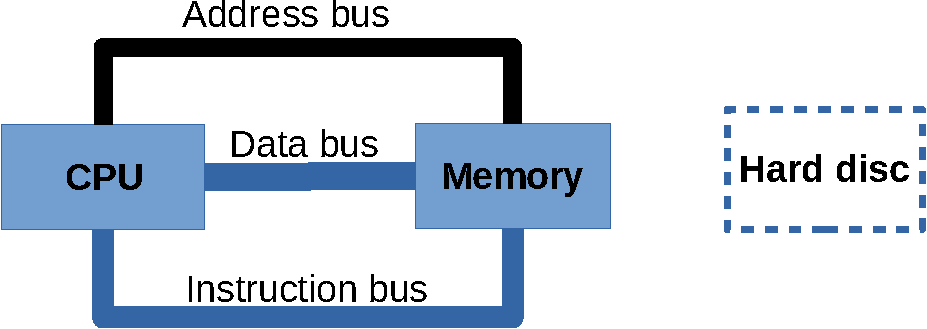
\includegraphics[width=0.7\linewidth]{figs/framework.pdf}
\end{figure}
\end{frame}

\begin{frame}
\frametitle{About Computer (5): who is who}
\begin{figure}
	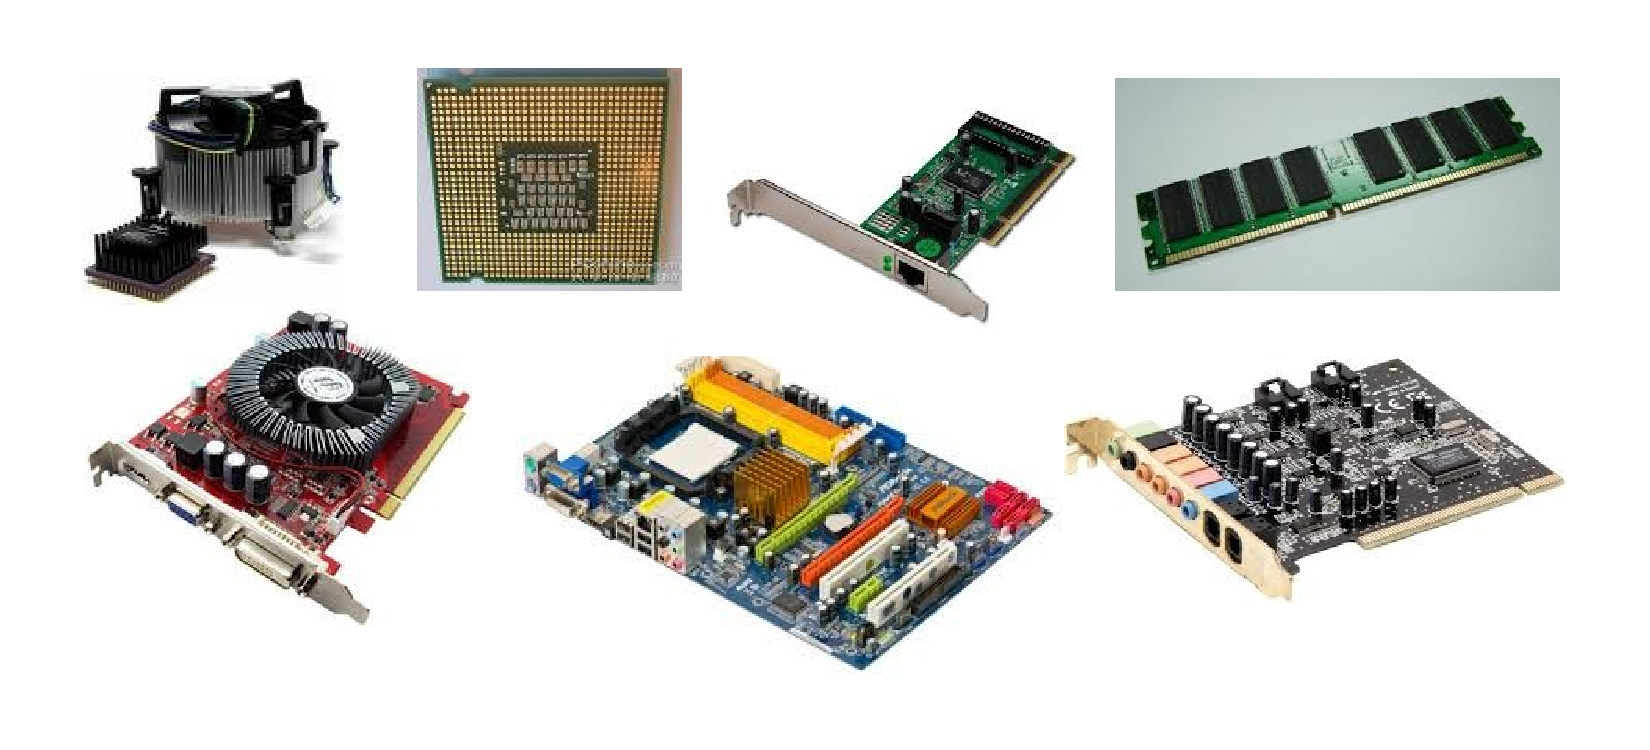
\includegraphics[width=0.85\linewidth]{figs/hardwares.pdf}
\end{figure}
\begin{itemize}
	\item {How many of them you can finger out?}
\end{itemize}
\end{frame}

\begin{frame}
\frametitle{About Computer (6): basic elements in Computer Chips}
\begin{figure}
	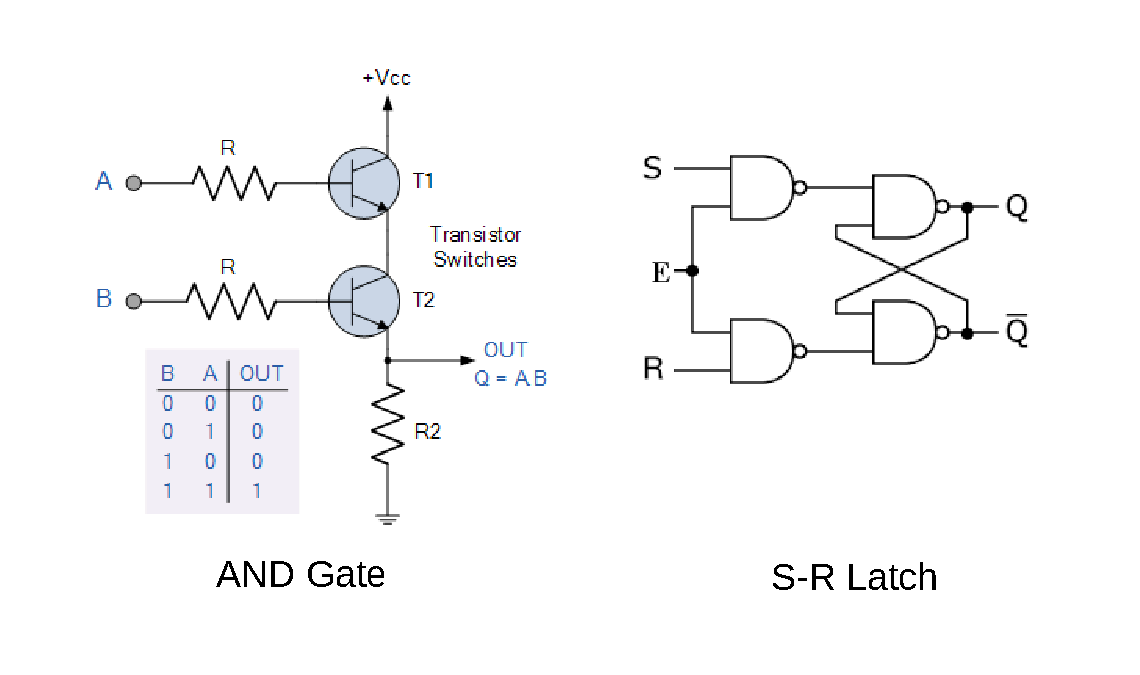
\includegraphics[width=0.6\linewidth]{figs/chips.pdf}
\end{figure}
\begin{itemize}
	\item {Despite the high complexity of VLSIC (very large scale integrated circuits)}
	\item {Only two basic elements are there}
	\item {One is gate, responsible for operations, main components for CPU}
	\item {Another is latch, in charge of memory, main components for memory}
\end{itemize}
\end{frame}